\documentclass{beamer}
\usepackage[utf8]{inputenc}
\usepackage[frenchb]{babel}
\usepackage[T1]{fontenc}
\usepackage{multicol}
\usepackage{lmodern}
\usepackage{vwcol}

\usetheme{Warsaw}

%\setbeamertemplate{headline}{}

\title[Rapport final de GRO]
      {Rapport final du projet de\\Graphes et Recherche opérationnelle}
\institute{Enseeiht}
\author
  [Ahlouche \and Arthaud \and Auguste
    \and Carton \and Forgione \and Wagner]
  {Maxence Ahlouche \and Maxime Arthaud \and Korantin Auguste
    \and Martin Carton \and Thomas Forgione \and Thomas Wagner}
\date{17 décembre 2013}

\newcommand{\brokencell}[2][c]{\begin{tabular}[#1]{@{}c@{}}#2\end{tabular}}

\begin{document}

\begin{frame}
  \titlepage
\end{frame}

\section{Graphes}

\subsection{Graphes eulériens}
\begin{frame}{Graphes eulériens}
  \begin{itemize}
    \item Cycle eulérien: cycle parcourant toutes les arêtes du graphe une et une seule fois
    \item Chaîne eulérienne: idem, mais ne retourne pas au sommet de départ
    \item Graphe eulérien: graphe contenant un cycle eulérien (degré des sommets toujours pair)
    \item Graphe semi-eulérien: graphe contenant une chaîne eulérienne (degré des sommets toujours pair, sauf pour les extrémités de la chaîne eulérienne)
  \end{itemize}
\end{frame}

\begin{frame}{Graphes eulériens}
  Matrices latines
  \begin{itemize}
  \item Teste toutes les possibilités
  \item Très peu efficace
  \end{itemize}
  Algorithme d'Euler
  \begin{itemize}
  \item Cherche des cycles eulériens dans des sous-graphes, récursivement
  \item Beaucoup plus efficace
  \end{itemize}
\end{frame}

\subsection{Graphes hamiltoniens}
\begin{frame}{Graphes hamiltoniens}
  \begin{itemize}
    \item Cycle hamiltonien: cycle parcourant tous les sommets du graphe une et une seule fois
    \item Chaîne hamiltonienne: idem, mais ne retourne pas au sommet de départ
    \item Graphe hamiltonien: graphe contenant un cycle hamiltonien
    \item Graphe semi-hamiltonien: graphe contenant une chaîne hamiltonienne 
    \item Pas de propriété générale pour déterminer si un graphe est hamiltonien ou non 
    \item NP-complet: pas d'algorithme efficace
  \end{itemize}
\end{frame}

\subsection{Voyageur de commerce}
\begin{frame}{Voyageur de commerce -- Énoncé}
    Chercher un chemin passant par tous les sommets, de longueur minimale.
    \begin{itemize}
        \item cycle hamiltonien de coût minimal
        \item NP-complet
        \item méthodes approchées
    \end{itemize}
\end{frame}

\begin{frame}{Voyageur de commerce -- Résolution approchée}
    \begin{block}{Heuristiques}
        Aller sur le sommet le plus près
    \end{block}

    \begin{block}{Recherche locale~: 2-opt}
      \centering
      \begin{multicols}{2}
        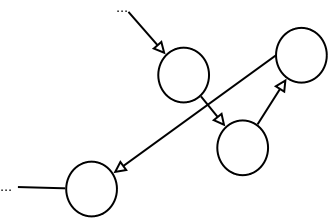
\includegraphics[width=0.3\textwidth]{../rapport/graphes/2opt1.png}

        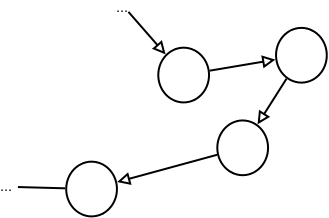
\includegraphics[width=0.3\textwidth]{../rapport/graphes/2opt2.png}
      \end{multicols}
    \end{block}
\end{frame}

\begin{frame}{Voyageur de commerce -- Tests}{}
    {\tiny
    \begin{table}[h]
      \makebox[\textwidth]{%
      \centering
      \begin{tabular}{| c | c | c | c | c | c |}
      \hline
        \brokencell{Fichier de\\test}
      & \brokencell{Résultat\\optimum}
      & \brokencell{Plus proche\\voisin}
      & \brokencell{Plus proche\\voisin + 2-opt}
      & \brokencell{Plus proche\\voisin amélioré}
      & \brokencell{Plus proche\\voisin amélioré\\+ 2-opt}\\
      \hline
      berlin52.tsp & $7542$  & $8981/19.1\%$ & $8060/6.7\%$ & $7972/5.7\%$ & $7810/3.6\%$ \\
      bier127.tsp & $118282$  & $137297/16.7\%$ & $125669/6.2\%$ & $127857/8.1\%$ & $122072/3.2\%$ \\
      d657.tsp & $48912$  & $62176/27.1\%$ & N/A & N/A & N/A \\
      u724.tsp     & $41910$ & $55344,32.1\%$ & N/A & N/A & N/A \\
      fl1577.tsp & $22249$  & N/A & N/A & N/A & N/A \\
      \hline  
      \end{tabular}
      }
      \caption{Résultats pour TSP}
    \end{table}
    }

    \url{http://www.iwr.uni-heidelberg.de/groups/comopt/software/TSPLIB95/}
\end{frame}

\begin{frame}{Voyageur de commerce -- Métaheuristiques}
    \begin{itemize}
        \item Recherche locale itérée
        \item Recherche tabou
        \item Recuit simulé
        \item Algorithmes génétiques
        \item Colonies de fourmis
    \end{itemize}
\end{frame}

\subsection{Postier chinois}
\begin{frame}{Postier chinois -- Énoncé}
  Trouver la chaîne la plus courte dans un graphe connexe passant au moins 
  une fois par chaque arête, et revenant à son point de départ.
\end{frame}

\begin{frame}{Postier chinois -- Méthode de résolution}
  \begin{enumerate}
    \item On crée d'abord le graphe partiel contenant uniquement les sommets
      de degré impair;
    \item On transforme ensuite ce graphe en clique;
    \item On cherche le couplage parfait de coût minimum;
    \item Pour chaque arête de cet ensemble, on double la chaîne la plus
      courte reliant les sommets reliés par cette arête dans le graphe initial;
    \item On applique l'algorithme d'Euler sur le graphe final.
  \end{enumerate}
\end{frame}

\section{Programmation linéaire}
\subsection{Sac à dos}
  \begin{frame}{Sac à dos -- Énoncé}
    Remplir un sac pour maximiser la valeur des objets, sans dépasser une
    certaine masse.
  \end{frame}

  \begin{frame}{Sac à dos -- Résolution}
    \begin{itemize}
      \item Résolution exacte:
      \begin{itemize}
        \item Programmation dynamique.
        \item Masses entières uniquement.
        \item $O(nW)$
      \end{itemize}

      \item Résolution dynamique:
      \begin{itemize}
        \item Algorithme glouton.
        \item Masses quelconques.
        \item $O(n \log n)$
      \end{itemize}
    \end{itemize}
  \end{frame}

  \begin{frame}{Sac à dos -- Résultats}{}
    {\tiny
    \begin{table}[h]
      \makebox[\textwidth]{%
      \centering
      \begin{tabular}{| c | c | c | c | c | c |}
      \hline
        \brokencell{Nombre d'objets/\\
                    Amplitudes des prix et masses/\\
                    Masse maximale autorisée}
      & \brokencell{Résultat\\optimum}
      & \brokencell{Prix le\\plus élevé}
      & \brokencell{Masse la\\plus faible}
      & \brokencell{Meilleur ratio\\prix/masse}\\
      \hline
      50/25/20& $85$ & $49/42.4\%$ & $67/21.2\%$ & $81/4.7\%$ \\
      500/25/500& $2016$ & $1125/44.2\%$ & $1725/14.4\%$ & $1983/1.6\%$ \\
      5000/25/500& $5540$ & $1175/79\%$ & $4577/17.4\%$ & $5540/0\%$ \\
      50000/25/500& $11195$ & $1175/90\%$ & $6684/40.3\%$ & $11195/0\%$ \\
      50000/1000/500& $118260$ & $5959/95\%$ & $101857/13.9\%$ & $118147/0.1\%$ \\
      50000/5000/100& $100847$ & $14931/85.2\%$ & $93532/7.3\%$ & $100282/0.6\%$ \\
      \hline  
      \end{tabular}
      }
      \caption{Résultats pour le sac à dos}
    \end{table}
    }

    \url{http://www.diku.dk/~pisinger/codes.html}
  \end{frame}

\subsection{Simplexe}
  \begin{frame}{Simplexe -- Présentation du problème}
    \[\max_{x \in \mathbb{R}^n \atop Ax \leqslant b} f(x)\]
    \begin{exampleblock}{Exemple}
      \begin{center}
        \begin{tabular}{|c|cccc|c|}\hline
          & $P_1$ & $P_2$ & $P_3$ & $P_4$ & stock \\ \hline
          $R_A$ & 2 & 4 & 5 & 7 & 72 \\
          $R_B$ & 1 & 1 & 2 & 2 & 17 \\
          $R_C$ & 1 & 2 & 3 & 3 & 24 \\ \hline
          bénéfice & 7 & 9 & 18 & 17 &  \\ \hline
        \end{tabular}
      \end{center}
    \end{exampleblock}
  \end{frame}

  \begin{frame}{Simplexe -- Simplification du problème}
    Transformation des contraintes d'inégalité en égalité.

    \begin{exampleblock}{Exemple}
      \begin{center}
        \begin{tabular}{|c|ccccccc|c|}\hline
          & $P_1$ & $P_2$ & $P_3$ & $P_4$ & $x_1$ & $x_2$ & $x_3$ & stock \\ \hline
          $R_A$ & 2 & 4 & 5 & 7 & 1 & 0 & 0 & 72 \\
          $R_B$ & 1 & 1 & 2 & 2 & 0 & 1 & 0 & 17 \\
          $R_C$ & 1 & 2 & 3 & 3 & 0 & 0 & 1 & 24 \\ \hline
          bénéfice & 7 & 9 & 18 & 17 & 0 & 0 & 0 & \\ \hline
        \end{tabular}
      \end{center}
    \end{exampleblock}
  \end{frame}

  \begin{frame}{Simplexe -- Algorithme}
    \begin{block}{Algorithme}
      Tant qu'il y a un élément strictement positif sur la première ligne\\
      \quad à\_ajouter = indice de la colonne dont le gain est maximal \\
      \quad à\_retirer = $\underset{i}{\text{argmin}} \frac{
                      matrice[i, stock]}{matrice[i, \text{à\_ajouter]}}$ \\
      \quad mettre à\_ajouter dans la base et retirer à\_retirer de la base \\
      \quad mettre à jour le reste de la matrice \\
      Fin Tant que
    \end{block}

    \begin{block}{Cas difficiles}
      \begin{itemize}
        \item Cas où l'ensemble de départ vide
        \item Cas où $(0,0) \notin C$
        \item Cas de dégénérescence
      \end{itemize}
    \end{block}
  \end{frame}

  \begin{frame}{Simplexe -- Une itération}
    \begin{exampleblock}{Exemple}
      \begin{center}
        \begin{tabular}{|c|ccccccc|c|}\hline
          & $P_1$ & $P_2$ & $P_3$ & $P_4$ & $x_1$ & $x_2$ & $x_3$ & stock \\ \hline
          $R_A$ & 2 & 4 & 5 & 7 & 1 & 0 & 0 & 42 \\
          $R_B$ & 1 & 1 & 2 & 2 & 0 & 1 & 0 & 17 \\
          $R_C$ & 1 & 2 & 3 & 3 & 0 & 0 & 1 & 24 \\ \hline
          bénéfice & 7 & 9 & \color{red}18\color{black} & 17 & 0 & 0 & 0 & \\ \hline
        \end{tabular}
      \end{center}
    \end{exampleblock}
  \end{frame}

 \begin{frame}{Simplexe -- Une itération}

    \begin{exampleblock}{Exemple}
      \begin{center}
        \begin{tabular}{|c|ccccccc|c|}\hline
          & $P_1$ & $P_2$ & $P_3$ & $P_4$ & $x_1$ & $x_2$ & $x_3$ & stock \\ \hline
          $R_A$ & 2 & 4 & \color{blue}5\color{black} & 7 & 1 & 0 & 0 & 42 \\
          $R_B$ & 1 & 1 & \color{blue}2\color{black} & 2 & 0 & 1 & 0 & 17 \\
          $R_C$ & 1 & 2 & \color{red}3\color{black} & 3 & 0 & 0 & 1 & 24 \\ \hline
          bénéfice & 7 & 9 & \color{red}18\color{black} & 17 & 0 & 0 & 0 & \\ \hline
        \end{tabular}
      \end{center}
    \end{exampleblock}
  \end{frame}
\begin{frame}{Simplexe -- Une itération}

    \begin{exampleblock}{Exemple}
      \begin{center}
        \begin{tabular}{|c|ccccccc|c|}\hline
          & $P_1$ & $P_2$ & $P_3$ & $P_4$ & $x_1$ & $x_2$ & $x_3$ & stock \\ \hline
          $R_A$ & 1/3 & 2/3 & 0 & 2 & 1 & 0 & -5/3 & 2 \\
          $R_B$ & 1/3 & -1/3 & 0 & 0 & 0 & 1 & -2/3 & 1 \\
          $R_C$ & 1/3 & 2/3 & 1 & 1 & 0 & 0 & 1/3 & 8 \\ \hline
          bénéfice & 1 & -3 & 0 & -1 & 0 & 0 & -6 & -144 \\ \hline
        \end{tabular}
      \end{center}
    \end{exampleblock}
  \end{frame}

\section{Jeux}
\subsection{Shifumi}

\begin{frame}{Shifumi}
    \begin{block}{Équilibre de Nash}
        Équilibre de Nash~: jouer de manière aléatoire.
    \end{block}

    \begin{itemize}
        \item Chaines de Markov~: bat aisément un humain qui joue «~normalement~».
        \item Variantes~: reviennent au Shifumi classique si le nombre d'éléments est impair.
    \end{itemize}
\end{frame}

\subsection{Somme magique}
\begin{frame}{Somme magique}
  todo
\end{frame}

\subsection{Duopole}
\begin{frame}{Duopole -- principe}
  \begin{vwcol}[widths={0.6,0.4}, sep=.0cm, rule=0pt]
    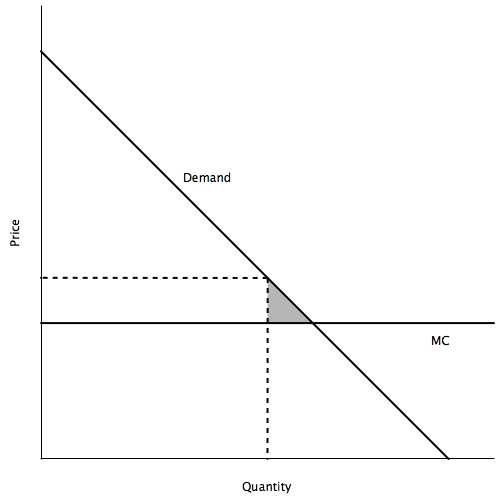
\includegraphics[width=0.55\textwidth]{jeux/duopole_principe}

    Nos stratégies:
    \begin{itemize}
      \item Stackelberg en moyenne \\
      $x=\frac{3-y}{2}$
      \item Stratégie pénalisante
      \item Stratégie évolutive
      \item Stratégie polynomiale \\
      $f(0) = 1.125$ \\
      $f(0.75) = 0.75$ \\
      $f(1.5) = 0.75$ \\
    \end{itemize}
  \end{vwcol}
\end{frame}

\begin{frame}{Duopole -- résultats}
  \tiny{%
    \begin{table}[f]
      \centering
      \begin{tabular}{|c||c|c|c|}
        \hline
        Stratégie      & Gain minimal & Gain moyen & Gain maximum \\\hline\hline
         cooperatif* & $561.56$ & $978.59$ & $1123.88$ \\\hline
      noncooperatif* & $380.79$ & $877.10$ & $1317.08$ \\\hline
        stackelberg* & $498.00$ & $797.42$ & $1132.44$ \\\hline
              palkeo & $694.54$ & $986.94$ & $1123.88$ \\\hline
            Pénalise & $419.12$ & $860.12$ & $1124.70$ \\\hline
   Pénalise variante & $421.22$ & $896.10$ & $1123.88$ \\\hline
Stackelberg en moyenne & $492.11$ & $923.94$ & $1123.88$ \\\hline
Stackelberg en moyenne (variante) & $531.85$ & $800.61$ & $1262.25$ \\\hline
            gklmjbse & $561.56$ & $832.41$ & $1135.33$ \\\hline
                poly & $561.82$ & $1011.24$ & $1123.88$ \\\hline
            killer** & $  0.00$ & $773.86$ & $1133.09$ \\\hline
   cooperatifmixte** & $698.67$ & $990.58$ & $1123.88$ \\\hline
    agressivemieux** & $  3.15$ & $750.64$ & $1126.18$ \\\hline
   best\_strategie** & $322.67$ & $881.00$ & $1262.81$ \\\hline
      \end{tabular}
      \caption{Résultats des différentes stratégies sur 1000 tours}
      \label{table:coop_results2}
    \end{table}
  }
\end{frame}

\section{Programmation stochastique}
\subsection{Gare de péage}
  \begin{frame}{Gare de péage}
    \begin{vwcol}[widths={0.6,0.4}, sep=.0cm, rule=0pt] 
      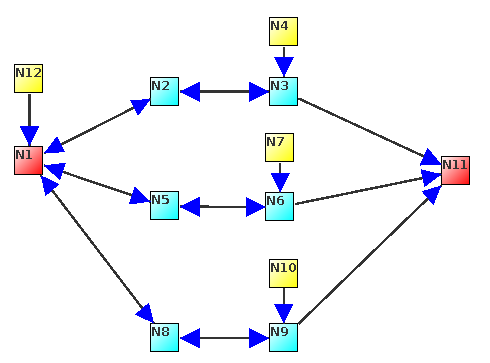
\includegraphics[width=6cm]{../../procstochs/img/3_files.png}

      \tiny
      \begin{itemize}
        \item $x[12] = random() < p_{cb}$
        \item $x[1] = random() < lambda$
        \item $x[2] =(x[2]>0)*(x[2]-1+d_{32})+d_{12}$
        \item $d_{12} = x[1]*d_{121}*(d_{21}<=d_{81})$
        \item $d_{23} = (x[2]>0)$
        \item $d_{32} = x[3]*(1-d_{43})$
        \item $x[3] = d_{23} + x[3]*(1-d_{23})*(1-d_{43})$
        \item $d_{311} = x[3]*d_{43}$
        \item $x[10] = random() < \frac 1 {p_{cb}/\mu_{cb}+(1-p_{cb})/\mu_{ncb}}$
      \end{itemize}
    \end{vwcol}
  \end{frame}

\section{Robots}
  \begin{frame}{UA 5 Robots}
      \begin{itemize}
          \item Suivi de mur
          \item Algorithme de Dijkstra
          \item Algorithme A*
      \end{itemize}
  \end{frame}
  \begin{frame}{Suivi de mur}
    Un capteur ultrasonique à gauche.

    Un capteur ultrasonique frontale.

    \begin{itemize}
      \item Si distance frontale < minima: on pivote à droite.
      \item Sinon:
      \begin{itemize}
        \item Si distance latérale > distance voulue + marge: coupe le moteur
        de gauche \\Sinon il est actif \item Si distance latérale < distance
          voulue - marge: coupe le moteur de droite \\Sinon il est actif
      \end{itemize}
    \end{itemize}
  \end{frame}

  \begin{frame}{Algorithme de Dijkstra}
    \begin{center}
      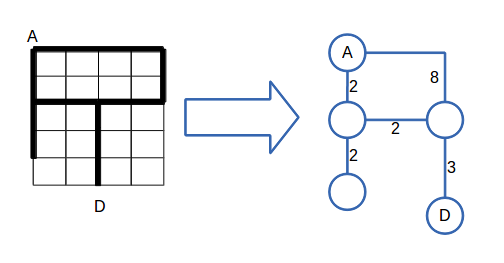
\includegraphics[width=0.55\textwidth]{jeux/GRO_graph1} \\
    \end{center}
    Si le robot connaît le plan du labyrinthe l'algorithme de dijkstra suffit. 
  \end{frame}
\end{document}
